\section{Design and Implementation of Frontend}

Our development journey began with a thorough analysis of the client’s requirements to ensure a clear understanding of the project goals and user needs. This foundational step allowed us to identify both functional and non-functional aspects critical to delivering a seamless multilingual virtual tour assistant. Following this, we carefully evaluated and selected the most suitable technologies to meet these requirements efficiently and maintainably. To visualize the user experience and interface, we created detailed wireframes and interactive prototypes using Figma, which facilitated early feedback and iterative improvements before moving into full development.

\subsection{Frontend Functional and Non-Functional Requirements}

\textbf{Note:} We need to decide whether this section will be here or elsewhere and we have not finalized the clear requirements.

The frontend requirements for Tourlingo were shaped by the needs of travelers, the feedback collected from early design iterations, and the overall goal of providing a seamless and engaging user experience. Since the frontend is the primary point of interaction, its design had to balance aesthetics, performance, and usability. \\ 

The most essential functional requirement was to provide a \textbf{clear and responsive user interface for real-time translation}. Users needed a simple way to input text through the search bar, where queries related to places, essentials, or recommendations could be entered. The results were then displayed on the map with the corresponding information instantly translated into the user’s chosen language. This ensured that searching and exploring cultural information on the map was intuitive and seamless. Because translation is the heart of Tourlingo, this requirement had the highest priority. In addition, the frontend was designed to support \textbf{multilanguage interfaces}, ensuring that the application itself (menus, buttons, and guidance) can adapt to the preferred language of the user.  \\

Another key requirement was the ability to handle \textbf{smooth communication with the backend APIs}. The frontend had to efficiently send translation requests and render responses almost instantly, minimizing waiting times. To achieve this, it was structured around \textbf{RESTful API integration}, using JSON payloads to keep the exchange consistent and lightweight.  \\

Since Tourlingo also provides cultural insights, the frontend was required to present this information in a \textbf{well-structured and engaging format}. Categories such as etiquette,  must-know phrases, payment methods, transportations, and emergency numbers were displayed using expandable sections, making the content accessible and digestible. To improve usability, components such as the \textbf{search bar} were designed to be \textbf{reusable}, ensuring consistency across different views such as the map and language pages.  

Finally, the \textbf{map-based interface} was developed to bring an interactive dimension/experience to the app. The pins on the map highlight key locations, while the dynamic side panels display contextual information. This combination turned the map into more than a visual element. It became an interactive tool for cultural orientation.  

\subsubsection{Non-Functional Requirements}

The non-functional aspects of the frontend were prioritized using the \textbf{MoSCoW methodology}, ensuring that the most critical user-facing qualities were delivered first.  

\textbf{Must Have:}  
\begin{itemize}
    \item \textbf{Responsiveness and performance:} Every screen needed to adapt gracefully to mobile, tablet, and desktop displays using a responsive design approach powered by Tailwind CSS. The frontend needed to display translated results almost immediately after a user request, so the experience felt seamless and gave the impression of real-time communication.

    \item \textbf{Usability and accessibility:}  The interface included a prominent search bar for entering text, intuitive language switching options, and consistent layouts across all screens. Accessibility was considered by ensuring readable font sizes, sufficient color contrast for map overlays, and keyboard navigation support, making the app usable by travelers with varying levels of digital literacy. \\
    \textbf{** shhhhh **}\\
    Clear navigation, consistent layouts, and adherence to accessibility guidelines ensured that the app could be used by travelers of different backgrounds and levels of digital literacy.  
\end{itemize}

\textbf{Should Have:}  
\begin{itemize}
    \item The interface should be designed with \textbf{scalability in mind}, so that new features (for example, adding cultural tips or new navigation tools) can be integrated later without requiring a complete redesign.  
    \item The system should provide \textbf{clear and user-friendly error handling}. For example, if a translation request fails or internet connectivity drops, the app should display an informative message rather than confusing the user.  
\end{itemize}

\textbf{Could Have:}  
\begin{itemize}
    \item An \textbf{offline first mode} could be introduced, where previously translated phrases or cultural notes are cached. This would allow travelers to access some functionality even without a stable Internet connection.  
    \item Subtle \textbf{animations and micro-interactions} could be added (such as smooth transitions when switching languages) to make the app feel more engaging and polished.  
\end{itemize}

\textbf{Won’t Have:}  
\begin{itemize}
    \item The frontend will not include \textbf{voice-to-text translation}, since it requires complex speech processing libraries and significant resources beyond the current scope of the project.  
    \item The app will not support \textbf{offline translation of entirely new inputs}, as this would require AI models on the device that are technically demanding and outside of the planned implementation.  
\end{itemize}

In summary, the frontend requirements for Tourlingo revolved around delivering a \textbf{clean, responsive, and intuitive interface that makes real-time translation and cultural learning effortless}. The non-functional requirements ensured that the system would remain robust, scalable, and pleasant to use, while consciously avoiding unnecessary complexity in the first release.


\subsection{Tech Stack Selection and Justification}

With a comprehensive understanding of the client's requirements, our next step was to carefully evaluate and select a technology stack that balances scalability, maintainability, performance, and developer experience. Each layer of the frontend architecture was considered through a comparative analysis of available tools and frameworks to ensure that the final selections were aligned with the long-term goals of the project.

\begin{table}[H]
\centering
\caption{Programming Language Comparison}
\begin{tabular}{|l|p{6cm}|p{6cm}|}
\hline
\textbf{Criteria}       & \textbf{JavaScript} & \textbf{TypeScript} \\
\hline
Typing                  & Dynamic             & Static             \\
Ease of Learning        & Easy                & Moderate           \\
Tooling Support        & Excellent           & Excellent          \\
Performance            & Good                & Good               \\
Reason                 & No static typing, harder to maintain large apps & Static typing improves code quality and maintainability \\
\hline
\end{tabular}
\label{tab:programming-language-comparison}
\end{table}

\textbf{Selected:} TypeScript \par
\textbf{Reasoning:} TypeScript was selected due to its static typing capabilities, which enhance code reliability, readability, and maintainability, especially for large-scale applications. Unlike JavaScript, TypeScript helps catch errors at compile time, making development more robust and reducing runtime bugs. It also offers better IDE support, including autocompletion and refactoring, improving developer productivity.

\vspace{2em}

\begin{table}[H]
\centering
\caption{Frontend Framework/Library Comparison}
\begin{tabular}{|l|p{4cm}|p{4cm}|p{4cm}|}
\hline
\textbf{Criteria}       & \textbf{React (Vanilla)}      & \textbf{Next.js}               & \textbf{Angular}               \\
\hline
Architecture            & Component-based UI library   & React-based framework with SSR/SSG & Full-featured MVC framework    \\
Ecosystem Size          & Very Large                   & Large (built on React)         & Large                          \\
Learning Curve          & Moderate                     & Moderate (extra SSR/SSG concepts) & Steep                          \\
Performance             & Excellent (CSR)              & Excellent (SSR + SSG options)  & Excellent                      \\
Flexibility             & High                         & Moderate (opinionated file structure) & Low                           \\
SEO Support             & Limited (CSR)                & Strong (built-in SSR \& SSG)   & Strong (built-in SSR)          \\
Reason                  & Great flexibility, simple setup & SEO benefits, server rendering, better routing & Steep learning curve, heavier structure \\
\hline
\end{tabular}
\label{tab:frontend-framework-comparison}
\end{table}

\textbf{Selected:} Next.js \par
\textbf{Reasoning:} Next.js was chosen for its built-in support for server-side rendering (SSR) and static site generation (SSG), which improve performance, search engine optimization (SEO), and initial load times. Its file-based routing simplifies navigation setup and integrates seamlessly with React’s component model. Compared to vanilla React, Next.js provides out-of-the-box optimizations and a more opinionated structure, reducing boilerplate. Angular, while powerful, was not selected due to its steeper learning curve, heavier framework size, and less flexibility for a React-focused tech stack.

\vspace{2em}

\begin{table}[H]
\centering
\caption{Styling Solutions Comparison}
\begin{tabular}{|l|p{4cm}|p{4cm}|p{4cm}|}
\hline
\textbf{Criteria}       & \textbf{CSS}               & \textbf{Tailwind CSS}        & \textbf{DaisyUI}             \\
\hline
Approach                & Traditional                & Utility-first                & Component-based              \\
Customizability         & High                       & Medium                      & Low                         \\
Learning Curve          & Easy                       & Moderate                    & Easy                        \\
Development Speed       & Moderate                   & Fast                        & Very Fast                   \\
Reason                  & Difficult to maintain large stylesheets & Rapid styling, consistent design system & Provides prebuilt components on Tailwind \\
\hline
\end{tabular}
\label{tab:styling-solutions-comparison}
\end{table}

\textbf{Selected:} Tailwind CSS + Daisy UI \par
\textbf{Reasoning:} Tailwind CSS was selected for its utility first approach, which accelerates development and enforces consistent styling across components. DaisyUI, built on top of Tailwind, adds ready-to-use, customizable UI components that speed up design implementation. This combination reduces the need to write custom CSS while keeping the UI modern and clean. Traditional CSS is harder to scale and maintain, and DaisyUI complements Tailwind without compromising flexibility.

\subsection{Implementation}

After finalizing the Figma prototype, the implementation phase commenced and was structured into iterative sprints. Each iteration focused on delivering incremental features, incorporating design feedback, and enhancing both performance and usability. The following sections provide a breakdown of the three main development iterations undertaken.

\subsubsection{Iteration 1:}
The first iteration focused on standing up a clickable skeleton aligned to the Figma user flows. The goal was to deliver a coherent theme, working navigation, language-scoped routing, page shells for all core areas.

\begin{enumerate}
    \item \textbf{Project Setup and Theme Baseline} \\
    Initialised the project with \texttt{Next.js (App Router)}, \texttt{React}, and \texttt{TypeScript} via \texttt{npm}. Established formatting and linting rules to reduce churn. Added \texttt{Tailwind CSS} and defined a global theme (colours, spacing, type scale) applied through \texttt{globals.css}.

    \item \textbf{Routing and Internationalisation} \\
    Introduced a language-scoped route segment \verb|app/[lang]/...|. Persisted the user’s language in \texttt{localStorage} so choices survive refreshes and deep links; URLs remain shareable in the chosen language.

    \item \textbf{Application Structure} \\
    Used App Router with feature folders to separate pages and reusable components.
    \begin{itemize}
        \item \textit{Pages:} \verb|[lang]/cultural-tips|, \verb|essentials|, \verb|language|, \verb|map|, \verb|recommendations|, plus \verb|layout.tsx| and \verb|page.tsx|.
        \item \textit{Components:} \texttt{NavigationBar}, \texttt{LanguageList}, \texttt{ActionButton}, \texttt{MapComponent}, \texttt{SearchBar}, \texttt{InfoAccordion}.
        \item \textit{Support:} \texttt{mockdata/}, \texttt{public/}, \texttt{types/}, \texttt{globals.css}.
    \end{itemize}

    \item \textbf{Reusable Components (v1)} \\
    Prioritised primitives used across pages:
    \begin{itemize}
        \item \textbf{NavigationBar} — top-level navigation mounted in \verb|app/layout.tsx|.
        \item \textbf{LanguageList} — renders supported languages; writes selection to \texttt{localStorage}.
        \item \textbf{ActionButton} — shared CTA styling (``Start'', ``Change language'').
        \item \textbf{MapComponent} — visual placeholder for the map view.
        \item \textbf{SearchBar / InfoAccordion} — early building blocks for dense content.
    \end{itemize}

    \item \textbf{Page Shells Delivered} \\
    Implemented page frames with one believable mock-driven page:
    \begin{itemize}
        \item \textbf{Language selector / Change language} — same component; CTA label differs; language persisted and reflected in \verb|[lang]|.
        \item \textbf{Cultural Tips} — basic prototype rendering tips from \texttt{mockdata/}; no geo logic or filtering yet.
        \item \textbf{Map} — page shell with \texttt{MapComponent} stub and placeholder panels.
        \item \textbf{Recommendations} — placeholder cards seeded from \texttt{mockdata/}.
        \item \textbf{Essentials} — placeholder sections 
    \end{itemize}

    \item \textbf{Styling and Layout} \\
    Tailwind utilities with a global layout (\verb|app/layout.tsx|) ensure a consistent frame; \texttt{NavigationBar} renders globally. Used Tailwind’s default breakpoints; finer responsive tweaks deferred until layouts stabilized.

    \item \textbf{State and Data} \\
    No backend integration in this iteration. Used mock data to validate layouts and interactions. Persistent state limited to language via localStorage.

    \item \textbf{Stakeholder Feedback} \\
    Positive response to being able to ``click around'' immediately. Cultural Tips showed too much text at once and felt basic; requested progressive disclosure and clearer grouping.

    \item \textbf{Outcome} \\
    Delivered a navigable app that matches Figma flows with a coherent theme, navigable skeleton with the language flow functional and a Cultural Tips page Map, Recommendations and Essentials were ready for data wiring and UX refinement in subsequent iterations.
\end{enumerate}

\subsubsection{Iteration 2:}
After completing the initial development in Iteration One, the second iteration focused on refining and enhancing the existing features based on testing and client feedback. The following key tasks were performed during this phase:

\begin{enumerate}
    \item \textbf{Bug Fixing from Previous Iteration} \\
    Several bugs identified in the first iteration were addressed. This included UI glitches, navigation issues, and minor functional problems. All fixes were thoroughly tested to ensure stability in the future.
    \item \textbf{Responsive Design Improvement} \\
    The entire application was reviewed and updated to ensure responsiveness between devices. Tailwind CSS utilities were used to make all pages and components adapted smoothly to various screen sizes, including mobile, tablet, and desktop.
    \item \textbf{Reusable Search Bar Component} \\
    The search bar that was originally built for the language selection page was converted to a generic reusable component. This allowed it to be used on the map page and potentially in other parts of the application, promoting code reuse and consistency.
    \item \textbf{Map Pins Integration} \\
    Pins were added to the map to represent important locations. This increased the interactivity of the map and provided users with visual cues linked to actual data and categories.
    \item \textbf{Dynamic Side Panels for Essentials and Recommendations} \\
    The static Essentials and Recommendations sections were redesigned as side panels. These panels now fetch real data from the backend API and display it with improved visual styling. Categories were introduced to organize the content better and make the user experience more intuitive.
    \item \textbf{Loading Animation for Backend Data Fetching} \\
    To enhance the user experience during interactions with the backend, a modern loading animation from \cite{uiverse-loader} was integrated. This provides clear visual feedback while waiting for data from the server (e.g. recommendations, essentials, and cultural tips), ensuring that users are informed of ongoing background processes and preventing the perception of lag.

    \item \textbf{Refining Cultural Tips}
    \begin{itemize}
        \item \textbf{Styling:} Several design mock-ups were presented to the client, and the final design was selected based on their feedback. The chosen layout was implemented with improved styling for better visual appeal.
        \item \textbf{Content Restructuring:} The earlier content was long and descriptive. It was revised and divided into clear and digestible sections on the basis of client's input. The final sections include:
        \begin{itemize}
            \item Etiquette
            \item Must-know Phrases
            \item Payment Methods
            \item Transportation
            \item Emergency Numbers
        \end{itemize}
    \end{itemize}
\end{enumerate}

\subsubsection{Iteration 3:}
This iteration focused on making the app feel faster, more reliable, easier to read at a glance, and friendlier for first-time users.

\begin{enumerate}
    \item \textbf{Map state management} \\
    Previously, when users navigated between pages, the map was automatically updated to their current location. This disrupted the user experience, especially if they were exploring a different area or had selected a destination.  

    We introduced a persistent \texttt{zustand} \cite{zustand-docs} store to manage all key map variables: user’s current location, selected destination, city, country, zoom level and searched text. The map state is now preserved across page navigations.  

    Users now return to the exact map view they left, maintaining continuity and improving usability. This makes exploration more intuitive and reduces frustration caused by unexpected recentering.


    \item \textbf{Preloading Cultural Tips (lightweight caching)} \\
    We now fetch cultural tips as soon as the city/language is known and keep a recent copy in a small local cache (zustand \cite{zustand-docs}). Returning users see tips immediately, while fresh data quietly replaces the cached copy in the background.

    \item \textbf{Tips that survive a reload} \\
    Previously, refreshing the page cleared the tips because they lived only in the component state. We moved them into a persistent \texttt{zustand \cite{zustand-docs}} store (backed by \texttt{localStorage}) and rehydrate on app load. Now, tips are available immediately after reload and refresh in the background once the location is confirmed.

    \item \textbf{Clearer map pins} \\
    The map uses distinct markers for (a) the current location of a user, (b) the selected destination and (c) each category in \emph{Recommendations} and \emph{Essentials}. This makes it easier to scan the map and match items in the side panel with what you see on the map.

    \item \textbf{First-time guide (intro.js)} \\
    A short, step-by-step walk-through (via \texttt{intro.js} \cite{introjs-docs}) introduces the basics: choose a language, explore the map, open essentials/recommendations, and view cultural tips. It appears only on first launch and is controlled by a simple \texttt{localStorage} flag.

    \item \textbf{Point-to-point directions (walk/cycle/drive)} \\
    We added directions from the user’s location to a searched or selected place for walking, cycling, and driving, each displayed in a unique color. For each route, the app now displays the estimated distance and the time required to cover it via the selected mode of transport. In addition, a static set of step-by-step directions is shown in a side panel, allowing users to easily follow the route without interacting with the map. Public-transport routing remains out of scope for this release.

    \item \textbf{Responsive UI improvements for map controls} \\
    On smaller devices, the map zoom-in and zoom-out buttons are used to overlap with the search bar and navigation bar. We update the layout so that the zoom controls reposition dynamically on the basis of screen size, ensuring that they remain accessible without obstructing other elements.
\end{enumerate}

\noindent\textbf{Outcome.} Users now return to the exact map view they left due to the persistent map state. Cultural tips load instantly on return visits and survive page reloads. The map pins are easier to interpret at a glance and first-time users receive a gentle guided tour of the core features. Basic point-to-point directions are available for walking, cycling, and driving. Additionally, the map controls are now responsive, with zoom buttons dynamically repositioning on smaller devices to avoid overlap with the search and navigation bars.

\begin{figure}[H]
    \centering
    \fbox{
    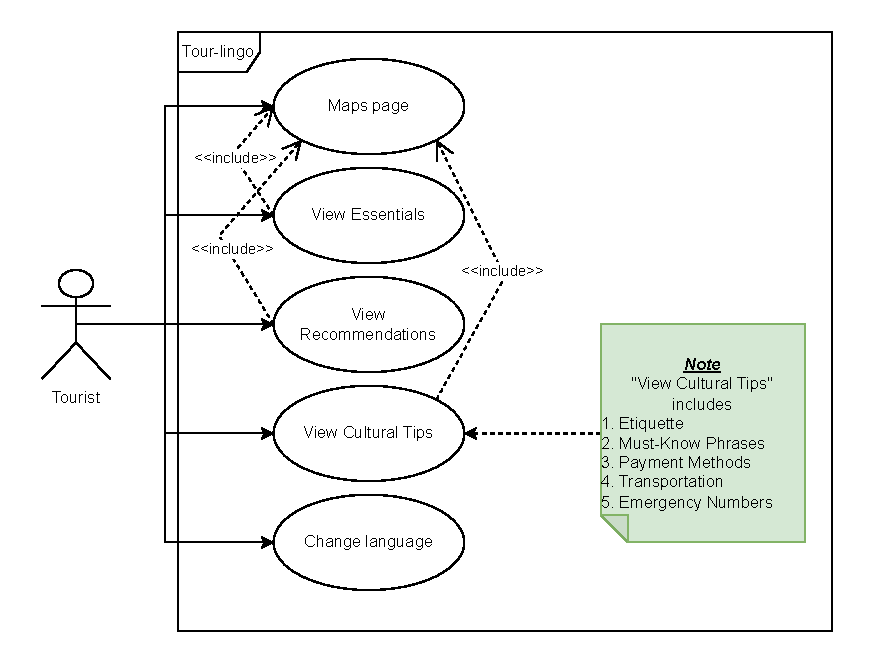
\includegraphics[width=0.5\linewidth]{images/Frontend/Frontend_Usecase_Diagram.pdf}
    }
    \caption{Frontend Use Case Diagram}
    \label{fig:frontend_usecase}
\end{figure}
